El filtro color consiste en realizar una iteracion sobre los pixeles de una imagen, estos se dividen en 3 componentes, cada una de ellas identifica un color de la codificacion RGB de la imagen. La iteracion del filtro deja sin modificaciones
los pixeles cuya distancia euclideana de sus componentes se encuentren dentro de un rango especificado por el par\'ametro threshold,los pixeles que no cumplan dicha condicion, se convertiran a blanco y negro por medio de una conversion basada en dejar las 3 componentes del pixel con el promedio de dichas componentes originales.
\\
\\
Como en esta ocasi\'on estamos trabajando con archivos de video, los cuales se pueden definir como una secuencia
de im\'agenes o frames. El filtro aplicar\'a frame por frame la operatoria explicada arriba como si fueran im\'agenes.
\\
\\
Dado que el objetivo de este trabajo pr\'actico es explorar el modelo de procesamiento SIMD que provee Intel, por este motivo se produjeron 2 implementaciones, una en lenguaje C, y la otra en ASM de 64 bits utilizando instrucciones SIMD.
\\

%%%%%%%%%%%%%%%%%%%%%%%%%%%%%%%%%%%%%%%%%%%%%%%%%%%%%%%%%%%%%%%%%%%%%%%%%%%%%%%
%% Descripción del ciclo                                                     %%
%%%%%%%%%%%%%%%%%%%%%%%%%%%%%%%%%%%%%%%%%%%%%%%%%%%%%%%%%%%%%%%%%%%%%%%%%%%%%%%

\subsubsection{Descripción del algoritmo}

Veamos la implementacion en C y utilizemosla como pseudocodigo para explicar el filtro:\\
Para cada frame del video de entrada, se realiza el siguiente algoritmo:\\

\lstinputlisting[language=C,tabsize=4, numbers=left, numberstyle=\tiny\color{black},mathescape=true, backgroundcolor=\color{gray}, rulecolor=\color{black}, keywordstyle=\color{blue}, commentstyle=\color{dkgreen},stringstyle=\color{mauve}, numbersep=5pt, basicstyle=\scriptsize]{fuentes/pseudocolor_filter_c.c}

\textbf{Explicacion del algoritmo:}\\ Dividamos en secciones el algoritmo en secciones y analicemos en detalle una por una.\\

\begin{enumerate}
    \item \textbf{Declaracion de variables : Lineas 15-25} \\
      Declaramos afuera del ciclo las variables que vamos a utilizar para el procesamiento.

    \item \textbf{Lectura de un pixel como 3 bytes desde la imagen origen : Lineas 26-30}\\
      Obtenemos de memoria los 3 bytes que corresponden a los colores azul, verde y rojo de un pixel.
      En la Figura se indica la lectura de este pixel.\\
      
      \par      
      \bigskip
        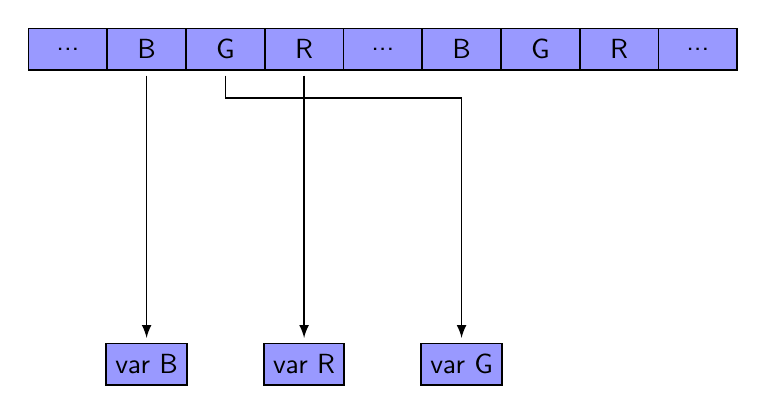
\begin{tikzpicture}
            [>=latex,font=\sffamily,every node/.style={minimum width=1cm,minimum height=1.5em,outer sep=0pt,draw=black,fill=blue!40,semithick}]
                    \node at (2, 0) (J) {var B};
                    \node at (4, 0) (L) {var R};
                    \node at (6, 0) (K) {var G};
            
            [>=latex,font=\sffamily,every node/.style={minimum width=1cm,minimum height=1.5em,outer sep=0pt,draw=black,fill=blue!40,semithick}]
                    \node at (1,4) (A) {...};
                    \node [anchor=west] at (A.east) (B) {B};
                    \node [anchor=west] at (B.east) (C) {G};
                    \node [anchor=west] at (C.east) (D) {R};
                    \node [anchor=west] at (D.east) (E) {...};
                    \node [anchor=west] at (E.east) (F) {B};
                    \node [anchor=west] at (F.east) (G) {G};
                    \node [anchor=west] at (G.east) (H) {R};
                    \node [anchor=west] at (H.east) (I) {...};

            
            %flechitas  
            \draw [->,shorten >=2pt,shorten <=2pt,semithick] (B.south) -- +(0,-1em) -| (J.north);
            \draw [->,shorten >=2pt,shorten <=2pt,semithick] (D.south) -- +(0,-1em) -| (K.north);
            \draw [->,shorten >=2pt,shorten <=2pt,semithick] (C.south) -- +(0,-1em) -| (L.north);
        \end{tikzpicture}

        \par
        \bigskip
        \textbf{Figura:} Lectura de un pixel en 3 variables componentes.
    \item \textbf{Procesamiento para obtener la distancia euclidiana : Lineas 31-39}\\
      Realizamos las operaciones aritmeticas necesarias sobre las 3 componentes del pixel obteniendo la distancia euclidiana. Para esta seccion se realizaron algunas conversiones de datos, a continuacion de justificaran las elecciones de variables.
      \\
      \begin{itemize}
        \item \textbf{Almacenamiento en double words: }
        Como la diferencia de dos bytes no signados puede estar en el rango
        [-255,255] necesitamos un tamaño de datos mas grande para contener este
        resultado, por ejemplo signed short(word). Se eligio utilizar variables
        signadas double word, pues luego, cuando se calcula el cuadrado, dicho numero
        puede tomar como maximo el valor 65535, que no podria representarse en un word signado.
        La distancia se almacena en double word pues como maximo puede tomar el valor 3*65535.
      \end{itemize}
    \item \textbf{Comparacion y procesamiento correspondiente: Lineas 40 y 47}\\
      Se realiza la comparacion entre la distancia calculada y el parametro umbral dado como par\'ametro, se decide por cual de las siguientes 2 etapas continuar el procesamiento.
    \item \textbf{Procesamiento Caso 1: Lineas 41-46}\\
      Esta seccion es ejecutada en caso de que la distancia euclidiana este fuera del rango de filtrado. Puede caracterizarse por la transformacion a blanco y negro de los pixeles que sean procesados por esta seccion.
      La conversion se realiza por medio de el calculo del promedio de las componentes del color del pixel, y la posterior
      escritura de dicho pixel dejando el promedio en cada una de las 3 componentes.
      Para esta seccion se realizaron algunas conversiones de datos, a continuacion de justificaran las elecciones de variables.
      \\
      \begin{itemize}
        \item \textbf{Variable auxiliar promedio y reconversion a byte sin signo: }
        Se expreso la variable promedio como un word sin signo, ya que alcanza para almacenar la suma maxima de 3 bytes no signados.\\
        Utilizando el siguiente lema, podemos asegurar que el promedio de 3 bytes no signados puede almacenarse como byte no signado, lo que nos permite una conversion segura de word sin signo a byte sin signo.\\
        \textbf{Lema: } Sea $ A = \{a_1, a_2, a_3, ... a_n\} $ un conjunto de bytes sin signo. Luego vale que $promedio(A) \leq max(A)$.
      \end{itemize}
    \item \textbf{Procesamiento Caso 2: Lineas 48-50}\\
      Esta seccion es ejecutada en caso de que la distancia euclidiana se encuentre dentro del rango establecido por el umbral. Consiste en escribir en destino el pixel de la misma forma que fue leido, sin modificaciones.
           
\end{enumerate}

Luego de realizar el algoritmo en C, se le aplicaron una serie de optimizaciones, a saber:
\begin{enumerate}
  \item \textbf{Eliminacion de llamadas innecesarias dentro del ciclo:} 
          Una temprana implementacion del filtro contenia la logica de la distancia tal cual especificada en el enunciado, y se encontraba plasmada en una funcion auxiliar que recibia los parametros y devolvia la distancia.
          Con el fin de eliminar saltos innecesarios dentro del ciclo, se decidio introducir esta funcion dentro del ciclo.
  \item \textbf{Eliminacion del calculo de la raiz cuadrada en cada ciclo: }
          Una temprana implementacion calculaba la distancia y la comparaba con el parametro threshold (o umbral) pasado por parametro. Se decidio elevar al cuadrado ambos miembros de la desigualdad, de forma que con calcular $threshold^2$ fuera del ciclo, y comparar con la distancia al cuadrado, se reducia la cantidad de calculos aritmeticos realizados.
  \item \textbf{Declaracion de variables auxiliares(de pila) fuera del ciclo}
          Una temprana temprana implementacion declaraba las variables auxiliares dentro del ciclo, se decidio declararlas fuera, de forma que con una sola declaracion con un scope mas general de las mismas se puedan reutilizar.

\end{enumerate}

\subsubsection{Implementacion en assembler utilizando set de instrucciones SIMD}

Para realizar esta implementacion se tomo la idea general de la implementacion en C, 
pero dada la naturaleza de la implementacion de SIMD se eliminaron los saltos condicionales, y se utilizaron mascaras para procesar los casos de aplicacion del filtro sobre los pixeles.\\
Se procesaran 4 pixeles por ciclo.\\

Dividamos en secciones el codigo y expliquemos cada una de ellas.\\

\begin{itemize}
  \item \textbf{Declaracion de mascaras y precomputo de calculos auxiliares}

            \par      
            \bigskip
             \begin{figure}[!ht]
              \centering
                 \begin{tikzpicture}
                  \registroDieciseis{}{0}{5}
                   {255}{255}{255}{9} {255}{255}{255}{6}
                   {255}{255}{255}{3} {255}{255}{255}{0}
              \end{tikzpicture}
              \caption{Mascara de reordenamiento de canal azul}
            \end{figure}


            \par      
            \bigskip
             \begin{figure}[!ht]
              \centering
                 \begin{tikzpicture}
                  \registroDieciseis{}{0}{5}
                   {255}{255}{255}{10} {255}{255}{255}{7}
                   {255}{255}{255}{4} {255}{255}{255}{1}
              \end{tikzpicture}
              \caption{Mascara de reordenamiento de canal verde}
            \end{figure}


            \par      
            \bigskip
             \begin{figure}[!ht]
              \centering
                 \begin{tikzpicture}
                  \registroDieciseis{}{0}{5}
                   {255}{255}{255}{11} {255}{255}{255}{8}
                   {255}{255}{255}{5} {255}{255}{255}{2}
              \end{tikzpicture}
              \caption{Mascara de reordenamiento de canal rojo}
            \end{figure}

            \par      
            \bigskip
             \begin{figure}[!ht]
              \centering
                 \begin{tikzpicture}
                  \registroDieciseis{}{0}{5}
                   {255}{255}{255}{255} {255}{255}{12}{255}
                   {255}{8}{255}{255} {4}{255}{255}{0}
              \end{tikzpicture}
              \caption{Mascara de reordenamiento inversa de canal azul}
            \end{figure}

            \par      
            \bigskip
             \begin{figure}[!ht]
              \centering
                 \begin{tikzpicture}
                  \registroDieciseis{}{0}{5}
                   {255}{255}{255}{255} {255}{12}{255}{255}
                   {8}{255}{255}{4} {255}{255}{0}{255}
              \end{tikzpicture}
              \caption{Mascara de reordenamiento inversa de canal verde}
            \end{figure}

            \par      
            \bigskip
             \begin{figure}[!ht]
              \centering
                 \begin{tikzpicture}
                  \registroDieciseis{}{0}{5}
                   {255}{255}{255}{255} {12}{255}{255}{8}
                   {255}{255}{4}{255} {255}{0}{255}{255}
              \end{tikzpicture}
              \caption{Mascara de reordenamiento inversa de canal rojo}
            \end{figure}            

        Estas mascaras de definen para los reordenamientos de los pixeles al comienzo y al final del ciclo.\\

        \textbf{Otros valores precalculados:}\\
      \begin{itemize}

        \item \textbf{THREE: } DB 3
        Esto se define de esta manera, y luego con instrucciones de mezclado y conversion se replica en un registro XMM como 4 floats empaquetados para realizar el calculo de la division por 3 en el promedio del blanco y negro.\\
            \par      
            \bigskip
             \begin{figure}[!ht]
              \centering
                 \begin{tikzpicture}
                  \registroCuatro{}{0}{5}
                   {3}{3}{3}{3}
              \end{tikzpicture}
              \caption{Mascara de constante 3 como 4 puntos flotantes de precision simple}
            \end{figure}  

        \item \textbf{Generacion de registros XMM con los parametros rc, bc, gc}
        Se definen 3 registros con 4 enteros de 32 bits empaquetados conteniendo replicados estos parametros, para realizar los calculos aritmeticos.\\
        \par      
        \bigskip
         \begin{figure}[!ht]
          \centering
             \begin{tikzpicture}
              \registroCuatro{}{0}{5}
               {RC}{RC}{RC}{RC}
          \end{tikzpicture}
          \caption{Mascara de constantes RC como 4 enteros de 4 bytes}
        \end{figure}  

        \par      
        \bigskip
         \begin{figure}[!ht]
          \centering
             \begin{tikzpicture}
              \registroCuatro{}{0}{5}
               {BC}{BC}{BC}{BC}
          \end{tikzpicture}
          \caption{Mascara de constantes BC como 4 enteros de 4 bytes}
        \end{figure}  

        \par      
        \bigskip
         \begin{figure}[!ht]
          \centering
             \begin{tikzpicture}
              \registroCuatro{}{0}{5}
               {GC}{GC}{GC}{GC}
          \end{tikzpicture}
          \caption{Mascara de constantes GC como 4 enteros de 4 bytes}
        \end{figure}  

        \item \textbf{Mascara con $threshold^2$}
        Se define esta mascara replicando como 4 floats empaquetados el valor de $threshold^2$.
                \par      
        \bigskip
         \begin{figure}[!ht]
          \centering
             \begin{tikzpicture}
              \registroCuatro{}{0}{5}
               {$threshold^2$}{$threshold^2$}{$threshold^2$}{$threshold^2$}
          \end{tikzpicture}
          \caption{4 floats empaquetados con el valor de $threshold^2$.}
        \end{figure}  

      \end{itemize}
      \par      
      \bigskip
  \item \textbf{Ciclo principal: Lectura de origen y reordenamiento de pixeles}
       \begin{figure}[!ht]
        \centering
          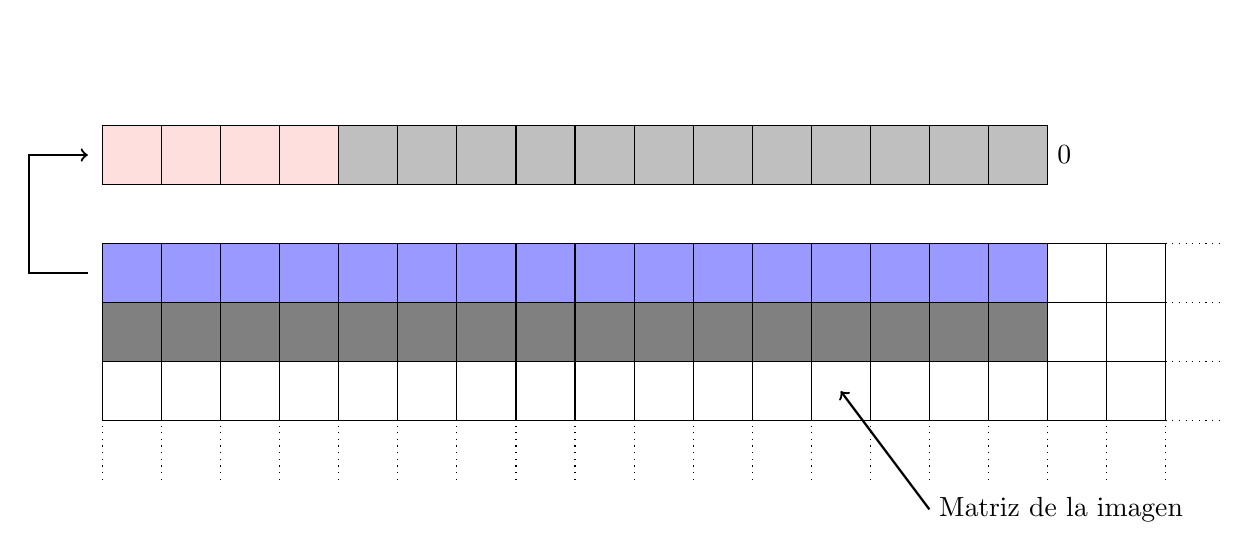
\begin{tikzpicture}[scale=0.75]
              \foreach \x in {0, ..., 4}
              {
                  % Registros
                  %\filldraw[fill=blue!40]      (\x, 8) rectangle +(1, 1);
                  \filldraw[fill=red!13] (\x, 6) rectangle +(1, 1);            

                  % Matriz
                  \filldraw[fill=blue!40]      (\x, 4) rectangle +(1, 1);
                  \filldraw[fill=gray]      (\x, 3) rectangle +(1, 1);

                  % Líneas de proyección inferiores
                  \draw                     (\x, 2) rectangle +(1, 1);
                  \draw [dotted] (\x, 1) -- +(0, 1) ++(1, 0) -- +(0, 1);
              }

              \foreach \x in {4, ..., 15}
              {
                  % Registros
                  %\filldraw[fill=blue!40]      (\x, 8) rectangle +(1, 1);
                  \filldraw[fill=lightgray] (\x, 6) rectangle +(1, 1);            

                  % Matriz
                  \filldraw[fill=blue!40]      (\x, 4) rectangle +(1, 1);
                  \filldraw[fill=gray]      (\x, 3) rectangle +(1, 1);

                  % Líneas de proyección inferiores
                  \draw                     (\x, 2) rectangle +(1, 1);
                  \draw [dotted] (\x, 1) -- +(0, 1) ++(1, 0) -- +(0, 1);
              }

              \foreach \x in {16, 17}
              {
                  % Matriz
                  \draw (\x, 4) rectangle +(1, 1);
                  \draw (\x, 3) rectangle +(1, 1);
                  \draw (\x, 2) rectangle +(1, 1);

                  % Líneas de proyección inferiores
                  \draw [dotted] (\x, 1) -- +(0, 1) ++(1, 0) -- +(0, 1);
              }

              \foreach \y in {2, ..., 5}
              {
                  % Líneas de proyección laterales
                  \draw [dotted] (18, \y) -- +(1, 0);
              }

              % Etiquetas de los registros
              \draw (16, 8.5) node[anchor=west]{}
                   +( 0,  -2) node[anchor=west]{\xmm{0}};

              % Etiqueta de la matriz
              \draw (14, 0.5) node[anchor=west]{Matriz de la imagen};
              \draw [->, thick] (14, 0.5) -- +(-1.5, 2);

              % Flechas entre registros
              \draw [->, thick] (-0.25, 4.5) -- ++(-1, 0)   -- ++(0, 2) -- +(1, 0);
              %\draw [->, thick] (-0.25, 4.5) -- ++(-0.5, 0) -- ++(0, 4) -- +(0.5, 0);

          \end{tikzpicture}
        \caption{Obtención de los 16 bytes (12 a procesar) en la iteración actual.}
        \label{pixeles}
      \end{figure}

      \textbf{Indice de colores de la figura anterior:}\\
      \begin{itemize}
        \item \textbf{Azul}
          Indica la porcion de memoria que se lee.\\
        \item \textbf{Gris}
          Indican las componentes que seran procesadas en este ciclo.\\
        \item \textbf{Rojo}
          Indican las componentes que seran descartadas en este ciclo y procesadas en el proximo.\\
      \end{itemize}

      Se leen los bytes indicados en la figura y se replican en \xmm{0}, \xmm{1}, \xmm{2}\\

      Luego se procede a reordenar los pixeles como se indica mas abajo.\\

      \par      
      \bigskip
       \begin{figure}[!ht]
        \centering
           \begin{tikzpicture}
            \registroDieciseis{}{0}{5}
             {x}{x}{x}{x} {$R_3$}{$G_3$}{$B_3$} {$R_2$}
             {$G_2$}{$B_2$} {$R_1$}{$G_1$}{$B_1$} {$R_0$}{$G_0$}{$B_0$}
        \end{tikzpicture}
        \caption{Contenido de los registros \xmm{ 0,1,2} antes del reordenamiento}
      \end{figure}

      \par      
      \bigskip
       \begin{figure}[!ht]
        \centering
         \begin{tikzpicture}
            \registroCuatro{\xmm{0}}{0}{5}
             {$B_3$} {$B_2$} {$B_1$} {$B_0$}
        \end{tikzpicture}
        \caption{Contenido del registro \textbf{AZUL} luego del reordenamiento con \textbf{PSHUFB} con la mascara correspondiente}
      \end{figure}

      \par      
      \bigskip
       \begin{figure}[!ht]
        \centering
           \begin{tikzpicture}
            \registroCuatro{\xmm{1}}{0}{5}
             {$G_3$} {$G_2$} {$G_1$} {$G_0$}
        \end{tikzpicture}
        \caption{Contenido del registro \textbf{VERDE} luego del reordenamiento con \textbf{PSHUFB} con la mascara correspondiente}
      \end{figure}

      \par      
      \bigskip
       \begin{figure}[!ht]
        \centering
           \begin{tikzpicture}
            \registroCuatro{\xmm{2}}{0}{5}
             {$R_3$} {$R_2$} {$R_1$} {$R_0$}
        \end{tikzpicture}
        \caption{Contenido del registro \textbf{ROJO} luego del reordenamiento con \textbf{PSHUFB} con la mascara correspondiente}
      \end{figure}
      \newpage


           Este reordenamiento pretende tener en los registros \xmm{0}, \xmm{1}, \xmm{2}, las componentes de los 4 pixeles a procesar en simultaneo como 4 enteros de 32 bits empaquetados.\\
      Luego de esta etapa, podremos realizar operaciones sobre 4 componentes de forma paralela con una sola instruccion gracias al set de instrucciones SIMD. Resguardo en \xmm{3}, \xmm{4}, \xmm{5} los registros \xmm{0}, \xmm{1}, \xmm{2} luego del reordenamiento, dado que los voy a modificar y necesito tener los originales en etapas mas.\\
  \item \textbf{Ciclo principal: Calculo de distancia euclidiana}\\
      \textbf{Nota inicial:} en representacion entera de 32 bits puedo realizar las restas, las elevaciones al cuadrado y las sumas sin problemas.\\
      En esta seccion, ya tenemos los pixeles organizados de forma tal que podemos realizar los siguientes calculos de forma empaquetada y en este orden:
        \begin{figure}[!ht]
              \centering
              \par      
              \bigskip
              \textbf{Operandos de la resta}
              \par      
              \bigskip
              \begin{tikzpicture}
                  \registroCuatro{}{0}{5}
                   {$R_3$} {$R_2$} {$R_1$} {$R_0$}
              \end{tikzpicture}
              \begin{tikzpicture}
                  \registroCuatro{}{0}{5}
                   {$RC$} {$RC$} {$RC$} {$RC$}
              \end{tikzpicture}  
            \par      
            \bigskip
            \textbf{Resultado de la resta}
            \par      
            \bigskip
            \begin{tikzpicture}
                \registroCuatro{}{0}{5}
                 {$(R_3$-$RC)$} {$(R_2$-$RC)$} {$(R_1$-$RC)$} {$(R_0$-$RC)$} 
            \end{tikzpicture}  
            \caption{Resta empaquetada ilustrativa entre 1 registro de componentes rojas y su parametro rc. Analogamente son las restas empaquetadas entre las componentes verdes y azules y sus parametros.}          
        \end{figure}
        
        \begin{figure}[!ht]
              \centering
              \par      
              \bigskip
              \textbf{Operandos del producto}
              \par      
              \bigskip
              \begin{tikzpicture}
                \registroCuatro{}{0}{5}
                 {$(R_3$-$RC)$} {$(R_2$-$RC)$} {$(R_1$-$RC)$} {$(R_0$-$RC)$} 
            \end{tikzpicture}  
              \begin{tikzpicture}
                \registroCuatro{}{0}{5}
                 {$(R_3$-$RC)$} {$(R_2$-$RC)$} {$(R_1$-$RC)$} {$(R_0$-$RC)$} 
            \end{tikzpicture}  
            \par      
            \bigskip
            \textbf{Resultado del producto}
            \par      
            \bigskip
            \begin{tikzpicture}
                \registroCuatro{}{0}{5}
                 {$(R_3$-$RC)^2$} {$(R_2$-$RC)^2$} {$(R_1$-$RC)^2$} {$(R_0$-$RC)^2$} 
            \end{tikzpicture}  
            \caption{Producto empaquetado de los registros por si mismos, de esta forma obtenemos las diferencias al cuadrado. Analogamente se realiza para las componentes verdes y azules.}          
        \end{figure}

        \begin{figure}[!ht]
              \centering
              \par      
              \textbf{Operandos de la suma}
              \bigskip
              \par  
              \begin{tikzpicture}
                  \registroCuatro{}{0}{5}
                   {$dr_3 = (R_3$-$RC)^2$} {$dr_2 = (R_2$-$RC)^2$} {$dr_1 = (R_1$-$RC)^2$} {$dr_0 = (R_0$-$RC)^2$} 
              \end{tikzpicture}
              \begin{tikzpicture}
                  \registroCuatro{}{0}{5}
                   {$db_3 = (B_3$-$BC)^2$} {$db_2 = (B_2$-$BC)^2$} {$db_1 = (B_1$-$BC)^2$} {$db_0 = (B_0$-$BC)^2$} 
              \end{tikzpicture}
              \begin{tikzpicture}
                  \registroCuatro{}{0}{5}
                   {$dg_3 = (G_3$-$GC)^2$} {$dg_2 = (G_2$-$GC)^2$} {$dg_1 = (G_1$-$GC)^2$} {$dg_0 = (G_0$-$GC)^2$} 
              \end{tikzpicture}
              \textbf{Resultado de la suma}
              \par      
              \bigskip
              \begin{tikzpicture}
                  \registroCuatro{}{0}{5}
                   {$(dr_3+db_3+dg_3)$} {$(dr_2+db_2+dg_2)$} {$(dr_1+db_1+dg_1)$} {$(dr_0+db_0+dg_0)$} 
              \end{tikzpicture} 
              
              \caption{Suma de las distancias de las 3 componentes de los pixeles. De esta forma obtenemos la distancia euclidiana al cuadrado. Notar que la suma es ilustrativa, pues la suma se realiza en 2 etapas, ver codigo.} 
        \end{figure}

        \newpage
  \item \textbf{Ciclo principal: Creacion de mascaras a partir de comparacion con umbral}
        En esta sección trabajaremos con punto flotante para realizar las comparaciones, ya que las instrucciones de punto flotante me permiten obtener de forma mas directa las mascaras que me indicaran que pixeles y cuales no deberan filtrarse. Realizo una comparacion por menor o igual entre las sumas y un registro conteniendo 4 veces threshold(ya precomputado fuera del ciclo).Asimismo realizo la comparacion inversa(not lower than) para obtener la mascara negada.

 \begin{figure}[!ht]
              \centering
              \par      
              \textbf{Comparación lower than threshold}
              \bigskip
              \par  
             \begin{tikzpicture}
                  \registroCuatro{}{0}{5}
                   {$(dr_3+db_3+dg_3)$} {$(dr_2+db_2+dg_2)$} {$(dr_1+db_1+dg_1)$} {$(dr_0+db_0+dg_0)$} 
              \end{tikzpicture}  
               \begin{tikzpicture}
                  \registroCuatro{}{0}{5}
                   {$threshold^2$} {$threshold^2$} {$threshold^2$} {$threshold^2$} 
              \end{tikzpicture}
              \textbf{Máscara resultado}
              \par      
              \bigskip
              \begin{tikzpicture}
                  \registroCuatro{}{0}{5}
                   {0xFFFFFFFF/00000000} {0xFFFFFFFF/00000000} {0xFFFFFFFF/00000000} {0xFFFFFFFF/00000000} 
              \end{tikzpicture}  
              \caption{Ejemplo de comparación lower than. Obtenemos una máscara con 0xFFFFFFFF ó 0x00000000 depediendo de si
              en esa posición, la suma de los cuadrados de las diferencias era menor o mayor o igual a threshold.} 
        \end{figure}

        
        En un etapa anterior habiamos replicado  en \xmm{3}, \xmm{4}, \xmm{5} los registros \xmm{0}, \xmm{1}, \xmm{2}, dado que durante el calculo de la distancia y la creacion de mascaras, destruimos los valores en \xmm{0}, \xmm{1}, \xmm{2}, en esta parte restituimos los valores destruidos y notando que las 2 mascaras son excluyentes al ser una la negacion de la otra las aplicamos sobre \xmm{0}, \xmm{1}, \xmm{2} y \xmm{3}, \xmm{4}, \xmm{5} respectivamente.
        De esta forma tenemos en cada tripla de registros (\xmm{0},\xmm{1},\xmm{2}) y (\xmm{3},\xmm{4},\xmm{5}) los 4 pixeles separados por componente y en en la primera tripla estan los que serán procesados a blanco y negro, mientras que en la segunda, se encuentran los que quedarán sin modificaciones. \\
        
\begin{figure}[!ht]
              \centering
              \par      
              \textbf{Aplicación de la máscara lower than en el registro ROJO}
              \bigskip
              \par  
             \begin{tikzpicture}
                  \registroCuatro{}{0}{5}
                   {$R_3$} {$R_2$} {$R_1$} {$R_0$} 
              \end{tikzpicture}  
               \textbf{(Máscara ejemplo)}
               \begin{tikzpicture}
                  \registroCuatro{}{0}{5}
                   {0xFFFFFFFF} {0x00000000} {0xFFFFFFFF} {0x00000000} 
              \end{tikzpicture}
              \textbf{Resultado:}
              \par      
              \bigskip
              \begin{tikzpicture}
                  \registroCuatro{}{0}{5}
                   {$R_3$} {0x00000000} {$R_1$} {0x00000000} 
              \end{tikzpicture}  
              \caption{Nos quedan los valores rojos de los pixeles que no tienen que cambiar, y 0s donde habia un valor rojo de un pixel que tiene que ser convertido a blanco y negro} 
        \end{figure}
        
        \newpage
        
  \item \textbf{Ciclo principal: Calculo de blanco y negro}      
        En esta seccion debemos realizar el calculo de promedio empaquetado entre los 3 registros de la tripla (\xmm{0},\xmm{1},\xmm{2}). Para ello realizamos sumas empaquetadas de enteros de 32 bits entre \xmm{0} y \xmm{1} y luego entre \xmm{0} y \xmm{2}, obteniendo las sumas en \xmm{0}. La division por 3 es realizada en punto flotante contra un registro precomputado que contiene la constante 3 replicada como 4 floats.\\
        \textbf{Nota:} Se realiza una conversion de entero de 32 bits a punto flotante simple antes de la division y una conversion inversa luego de esta.
        
        \begin{figure}[!ht]
              \centering
              \par      
              \textbf{Promedio de los componentes de los 4 pixeles}
              \bigskip
              \par  
             \begin{tikzpicture}
                  \registroCuatro{}{0}{5}
                   {$R_3$} {$R_2$} {$R_1$} {$R_0$} 
              \end{tikzpicture}  
            
			\begin{tikzpicture}
                  \registroCuatro{}{0}{5}
                   {$B_3$} {$B_2$} {$B_1$} {$B_0$} 
              \end{tikzpicture} 
              
              \begin{tikzpicture}
                  \registroCuatro{}{0}{5}
                   {$G_3$} {$G_2$} {$G_1$} {$G_0$} 
              \end{tikzpicture}   
              \bigskip          
            \textbf{Resultado de la suma}
               \begin{tikzpicture}
                  \registroCuatro{}{0}{5}
                   {$R_3$ + $B_3$ + $G_3$} {$R_2$ + $B_2$ + $G_2$} {$R_1$ + $B_1$ + $G_1$} {$R_0$ + $B_0$ + $G_0$} 
              \end{tikzpicture}
              \textbf{Conversión a float, división, y re-conversión a int}
              \par      
              \bigskip
              \begin{tikzpicture}
                  \registroCuatro{}{0}{5}
                   {$\frac{R_3 + B_3 + G_3}{3}$} {$\frac{R_2 + B_2 + G_2}{3}$} {$\frac{R_1 + B_1 + G_1}{3}$} {$\frac{R_0 + B_0 + G_0}{3}$} 
              \end{tikzpicture}  
              \caption{Obtenemos el promedio de las 3 componentes de cada pixel. Notar que este ejemplo es un caso en el cual todos los pixeles deben ser modificados} 
        \end{figure}
        
       \newpage 
  \item \textbf{Ciclo principal: combinacion de casos, reordenamiento de pixeles y escritura a destino}
        Esta seccion final, se encarga de combinar los 2 casos que habian quedado separados luego de aplicar las mascaras, y finalmente reordena las componentes de forma tal que queden en formato apropiado para ser escritas a destino. Notemos algunas cosas:
          \begin{itemize}
            \item \textbf{Los dos casos que se separan en la aplicacion de mascaras son disjuntos}\\
                  Por lo tanto con operaciones logicas de disyuncion, se pueden unificar.
            \item \textbf{Cuando se pasa un pixel a blanco y negro, las 3 componentes contienen el promedio}\\
                  Por lo tanto la unificacion entre los pixeles originales y el blanco y negro puede realizarse utilizando una sola componente del blanco y negro varias veces.

	   \begin{figure}[!ht]
              \centering
              \par      
              \textbf{Ejemplo de una unificación por medio de una operacion de disyuncion}
              \bigskip
              \par  
               \textbf{Registro de promedios}
             \begin{tikzpicture}
                  \registroCuatro{}{0}{5}
                   {$\frac{R_3 + B_3 + G_3}{3}$} {0x00000000} {$\frac{R_1 + B_1 + G_1}{3}$} {0x00000000} 
              \end{tikzpicture}  
            \bigskip
            
			 \textbf{Registro ROJO}
			\begin{tikzpicture}
                  \registroCuatro{}{0}{5}
                   {0x00000000} {$R_2$} {0x00000000} {$R_0$} 
              \end{tikzpicture}    
                 \bigskip         
            
            \textbf{Registro AZUL}
			\begin{tikzpicture}
                  \registroCuatro{}{0}{5}
                   {0x00000000} {$B_2$} {0x00000000} {$B_0$} 
              \end{tikzpicture} 
				 \bigskip              
              
              \textbf{Registro VERDE}
              \begin{tikzpicture}
                  \registroCuatro{}{0}{5}
                   {0x00000000} {$G_2$} {0x00000000} {$G_0$} 
              \end{tikzpicture}   
              \bigskip          
            \textbf{Luego del Packed OR:}
               
			 \textbf{Registro ROJO}
			\begin{tikzpicture}
                  \registroCuatro{}{0}{5}
                   {$\frac{R_3 + B_3 + G_3}{3}$} {$R_2$} {$\frac{R_3 + B_3 + G_3}{3}$} {$R_0$} 
              \end{tikzpicture}    
                 \bigskip         
            
            \textbf{Registro AZUL}
			\begin{tikzpicture}
                  \registroCuatro{}{0}{5}
                   {$\frac{R_3 + B_3 + G_3}{3}$} {$B_2$} {$\frac{R_3 + B_3 + G_3}{3}$} {$B_0$} 
              \end{tikzpicture} 
				 \bigskip              
              
              \textbf{Registro VERDE}
              \begin{tikzpicture}
                  \registroCuatro{}{0}{5}
                   {$\frac{R_3 + B_3 + G_3}{3}$} {$G_2$} {$\frac{R_3 + B_3 + G_3}{3}$} {$G_0$} 
              \end{tikzpicture}   
              \bigskip                
               
              \caption{Ya tenemos agrupadas y procesadas las componentes de los 4 pixeles. Lo único que queda ahora es hacer un reordenamiento de pixeles como el del principio, pero de manera inversa y finalmente escribir a destino el resultado} 
        \end{figure}
                  
          \end{itemize}
\end{itemize}
\newpage
\subsubsection{Optimizaciones y tecnicas especificas aplicadas a la implementacion con SIMD}
Se aplicaron las siguientes optimizaciones al codigo con el objetivo de mejorar la performance del filtro:
\begin{itemize}
    \item \textbf{Tecnica de desenrrollado de ciclo: }Esta tecnica se realizo mediante la aplicacion de una macro sobre el cuerpo del ciclo, y una adaptacion del ciclo original a uno que incluye 16 llamados a la macro, indicando el correspondiente desplazamiento relativo de la porcion de memoria a procesar, y la modificacion del incremento a los indices del ciclo correspondientes.
    De esta forma, se espera obtener una mejora en la performance dado que esta tecnica en teoria reduce 16 veces la cantidad de comparaciones que se realizan en la guarda del ciclo.
    \item \textbf{Optimizaciones heredadas de la implementacion C:} De la implementacion original en C, tomamos la idea de eliminar el calculo de la raiz cuadrada de la distancia euclidiana. 
    \item \textbf{Minimizacion de conversiones y operaciones con punto flotante: } Una temprana implementacion del filtro en assembler realizaba el $100\%$ de los calculos aritmeticos sobre 4 numeros empaquetados de punto flotante simple, luego nos dimos cuenta que esto ralentizaba mucho los calculos y la mayoria de ellos podian realizarse sobre enteros, dejando unicamente el calculo de mascaras por conveniencia de las instrucciones disponibles para el problema en el que estabamos trabajando, asi tambien la division empaquetada del promedio como un calculo necesario sobre punto flotante, se intento mejorar esto investigando una aproximacion de la division basada en multiplicar por una fraccion de la forma $\frac{j}{2^k}$ donde j,k son numeros enteros, de esta forma, podria realizarse una division con operaciones de producto por $j$ y un shift a derecha de $k$ lugares(division por $2^k$), pero tanto los errores de precision de la aproximacion como las complicaciones de modificacion del codigo y de operatoria paralela empaquetada que esto implicaba, hicieron que finalmente fuese descartada esta modificacion.
    \item \textbf{Reordenamientos y accesos a memoria: } Utilizamos reordenamientos de registros por medio de las instrucciones de \textbf{shuffle} para procesar los canales de los pixeles de la mejor forma que se nos ocurrio. Para la aplicacion de estas mascaras, utilizamos la mayor de cantidad de registros disponibles para evitar los accesos a memoria para datos estaticos, es decir, que no se modifican a medida que pasan los ciclos. Asi tambien, notando que 2 de las 3 las mascaras de reordenamiento inverso se pueden obtener realizando operaciones de corrimiento de bits de otra, se barajó la posibilidad de crear en cada ciclo dichas mascaras, evitando 2 de 3 accesos a memoria, sorprendentemente, los resultados numericos fueron peores realizando esto que manteniendo los 3 accesos, creemos que se debe a la memoria cache, por lo tanto descartamos esta ultima posibilidad.
\end{itemize}

\subsubsection{Analisis y resultados}
Luego de realizar la implementacion en assembler utilizando SIMD, comenzamos a realizar un analisis sobre las diferencias estructurales del codigo en ASM contra la implementacion en C, aprovechamos las opciones de compilacion con diferentes niveles de optimizacion que nos brinda el compilador \textbf{GCC} y para cada una de esas optimizaciones automaticas, realizamos una revision del codigo assembler generado con la herramienta \textbf{objdump}, lo cual nos permitio observar cuales son las optimizaciones que realiza cada nivel, cuales cosas mejoran, cuales se podrian continuar optimizando y de ser posible, como.\\
\par
Ademas, se realizo un experimento para poder ver el impacto de los saltos condicionales dentro de un ciclo, dicho analisis se realizo sobre la version del filtro en C, compilado con el primer nivel de optimizacion.

\subsubsection{Tiempos de ejecucion de diferentes experimentos}
\par
\textbf{Notas iniciales: }
Las mediciones se realizaron tomando dos promedios, el primero, es un promedio de los tiempos que toma cada llamada a la funcion particular del filtro a los k frames del video de entrada, esto nos dice cuantos ciclos consume en promedio la aplicacion del filtro a un frame. Luego ademas, se hace un promedio de la cantidad de veces o iteraciones que se aplica el filtro al mismo video. Creemos que es una buena medicion, ya que se diluyen los valores atipicos producto que produce el scheduler del sistema operativo al cambiar de contexto. Asi tambien pensamos que realizando la medicion de esta manera, sin tomar en cuenta el procesamiento de la libreria $OpenCV$para el procesamiento del archivo de video, es mas limpia y se centra mas en el analisis del codigo implementado.
\par
\bigskip
\textbf{Caracterizacion del experimento: }
\begin{itemize}
    \item \textbf{Iteraciones: } 10
    \item \textbf{Comando: } ./tp2 -t 10 -i $<implementacion>$ fcolor ink.avi 100 100 100 100
    \item \textbf{Nota:} Los experimentos de optimizaciones del compilador no suponen ninguna alteracion sobre el comando de testeo ya que se realizan sobre la compilacion de los fuentes C del filtro.
    \item \textbf{Nota 2:} El experimento sobre C.01 eliminando los saltos condicionales se realizo, dejando siempre por defecto la conversion a blanco y negro de los pixeles.
\end{itemize}
\par
\textbf{Resultados:}\\
\begin{center}
    \begin{tabular}{|l|l|l|l|l|l|l|l|}
        \hline
        Medición  & C.O0  & C.O1 ss & C.O1  & C.O2  & C.03  & ASM  & ASM LU \\
        \hline
        Ciclos por llamada & 21499106  & 2729604 & 6018971 & 5282602 & 5169947 & 3507714 & 3426934\\
        \hline
    \end{tabular}
\end{center}
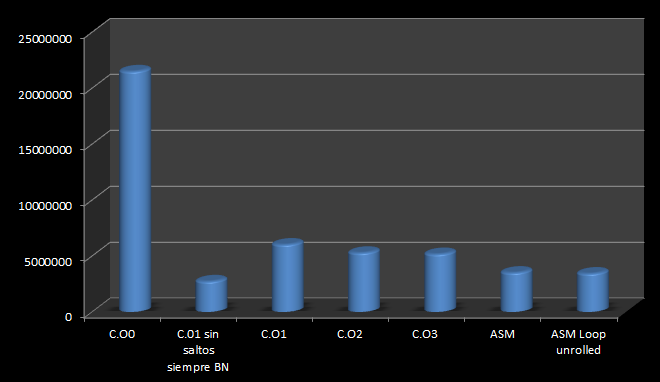
\includegraphics[scale=1]{imagenes/fcolor-grafico.png} 

\par
\bigskip
Una prueba adicional se hizo mientras se corria paralelamente un programa que utilizaba el 100\% del cpu arrojo resultados proporcionales. A continuacion de presentan en un grafico las relaciones entre las mediciones en estado $idle$ y en estado $100\%$ load.\\

\begin{center}
    \begin{tabular}{|l|l|l|l|l|l|}
        \hline
        Medición  & C.O0  & C.O1 & C.O2  & C.O3  & ASM LU  \\
        \hline
        Load & 33009164& 10239740  &7165908& 6709664 &4677277 \\
        \hline
        Idle & 21499106 & 6018971 & 5282602 & 5169947 & 3426934 \\
        \hline
        Relacion de incremento & 53\% & 70\% & 35\% & 30\% & 30\% \\
        \hline
    \end{tabular}
\end{center}
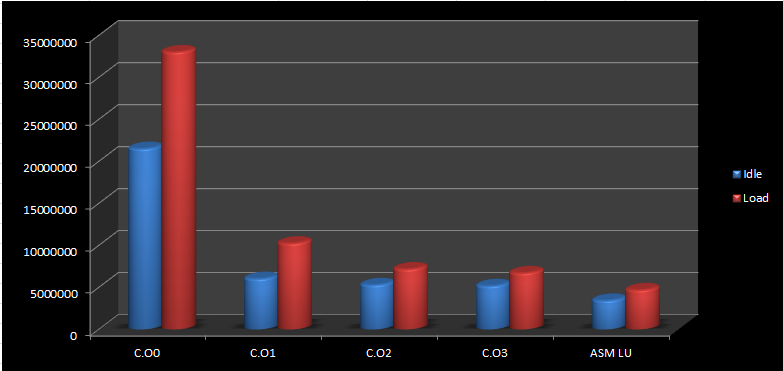
\includegraphics[scale=0.85]{imagenes/fcolor-grafico2.png} 

\subsubsection{Diferencias estructurales de las diferentes versiones analizadas}

En esta seccion nos centraremos en analizar las diferencias entre la version SIMD y las versiones C con sus diferentes niveles de optimizacion, de esta forma esperamos poder explicar los resultados numericos de la seccion anterior.
\\
\\
\textbf{Consideraciones iniciales:}\\
\par
Notoriamente entre la version del algoritmo en C y la version del algoritmo utilizando SIMD lo primero que hay que ver es que en la version de C se lee y procesa un pixel de origen por ciclo, mientas que utilizando SIMD, se procesan paralelamente 4 pixeles en instrucciones atomicas. Asi tambien cambia la forma de pensar el algoritmo como una division en casos con saltos condicionales entre ramificaciones de la ejecucion, hacia un pensamiento mas enfocado en procesamiento paralelo de valores, en los cuales mediante mascaras decidimos cuales componentes se procesaran con cada caso del filtro y luego, al ser casos disjuntos, pueden ser mezclados y escritos a destino, luego de realizar las conversiones y/o mezclados necesarios. 
\\
\textbf{Aclaracion sobre multiplicidad:} No tuvimos en cuenta los casos en donde la entrada tuviera un tamaño en pixeles que no fuera un multiplo de 4. Asumimos esta precondicion sobre la entrada para simplificar el algoritmo, podria solucionarse de forma sencilla sobre el codigo realizado, realizando un calculo de resto modulo 12 y una resta al puntero indice fuera del ciclo. Para informacion mas detallada de como solucionar este problema, dirigirse a la seccion del filtro \textbf{decode} donde se explica con mas detalle.
\\
\\
\textbf{Desensamblado de la implementacion original en C}\\
\par
Tomemos el codigo desensamblado con la herramienta \textbf{$objdump$} y busquemos posibles optimizaciones.
Podemos observar en el desensamblado del C sin optimizaciones, que las variables locales se utilizan como espacio de pila, produciendo un acceso a memoria cuando son requeridas para leer o escribir.Tambien afecta el traslado adicional entre memoria y registros para realizar operaciones.
\begin{center}
  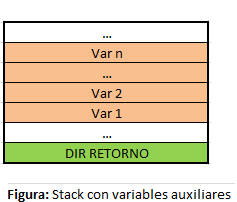
\includegraphics[scale=1]{imagenes/var-stack.png} 
\end{center}

Se encontro tambien la optimizacion en la division por 3 con el metodo de fraccion con denominador potencia de 2 mencionado anteriormente.

El resto del codigo parece acorde a la implementacion en C, de hecho es asi para permitir una correcta depuracion segun la documentacion de $GCC$.\\

Obviamente, el hecho de acceder a memoria para las variables locales, mas alla de lo que mejore la memoria cache, puede ser optimizado utilizando los registros internos del CPU y evitar estos accesos.\\
\\
\textbf{Incrementando la intensidad de la optimizacion: Primer nivel de optimizacion O1 }\\

En este modo se puede observar claramente el aprovechamiento de los registros internos del cpu para almacenar valores y variables temporales y evitar los accesos a memoria innecesarios. Asi tambien se observa que cambio el modo de direccionar la matriz ahora de una forma mas directa y con menor cantidad de instrucciones.

Es notorio el cambio en el tiempo de ejecucion este cambio, basta ver los graficos para ver que la reduccion considerable de accesos a memoria produjo una mejora importante.
\\
\\
\textbf{Analizando las optimizaciones mas agresivas:} O2 y O3\\
\par
$GCC$ nos ofrece una amplia variedad de flags para optimizar, se puede especificar en particular cada una de las posibles optimizaciones a realizar al codigo para obtener un ajuste fino. Por motivos de tiempo, solo analizaremos los flags que permiten optimizar de una forma automatica con cierto grado de agresividad, cada uno de estos flags engloba un grupo de optimizaciones particulares al codigo.
\\
\\
Un breve listado de las posibles optimizaciones estandares se muestra debajo:\\

\begin{center}
    \begin{tabular}{|l|l|}
        \hline
          Intensidad  & Descripcion\\
          \hline
          O0  & Casi ninguna transformacion al codigo, solo pasaje a assembler.  \\
          \hline
          O1  & Optimizaciones que no consuman mucho tiempo de compilacion.   \\
          \hline
          O2  & Optimizaciones que modifican el orden de ejecucion mejorando \\
           &  la velocidad del codigo resultante. Pueden verse alteradas variables \\
           &  del usuario y el cuerpo de algunas funciones.   \\
          \hline
          O3  & Optimizaciones que modifican aun mas el orden de ejecucion y pueden o no mejorar  \\
           &  la velocidad del codigo resultante. Puede verse alterada la semantica de las operaciones \\
           &  (particularmente las de punto flotante).\\
        \hline
    \end{tabular}
\end{center}

Existen otros parametros, entre ellos a saber $-Ofast$ que provee una mayor optimizacion que $-O3$ pero con el costo de no respetar los estandares. Por ejemplo, se implementa la optimizacion $ffast-math$ que acorde a la documentacion de $GCC$ puede producir errores en donde se espere una implementacion exacta del estandar IEEE o ISO de las funciones matematicas, es decir, puede verse alterada la precision de ciertos calculos.\\

Otro modo de optimizacion es $-Os$ que optimiza el tamaño del codigo manteniendo las optimizaciones de $-O2$ que no interfieran con el objetivo de este modo.\\

\textbf{Nota:} Para mas informacion dirigirse a:\\
\\
  \url{http://gcc.gnu.org/onlinedocs/gcc/Optimize-Options.html}\\
  \url{http://www.redhat.com/magazine/011sep05/features/gcc/}\\
\\

\subsubsection{Conclusiones acerca de las mediciones}
Luego de realizar estos analisis, podemos concluir acerca de las optimizaciones brindadas por el compilador $GCC$ que mejoran sorprendentemente la performance del mismo algoritmo, el mayor salto en rendimiento se ve con el primer nivel de optimizacion $O1$ que brinda el compilador. Asi mismo, la implementacion en assembler con SIMD obtiene mejores resultados que el C optimizado en su maximo nivel. El desenrrollado de ciclos brindo alguna mejora adicional, pero no demasiado significativa, y finalmente con respecto a los saltos condicionales, es muy notorio, como el procesador con su prediccion de saltos puede acelerar muchisimo la ejecucion, menos de la mitad de ciclos, ejecutando siempre la rama de ejecucion con mas costo, en este caso pasando siempre a blanco y negro realizando calculos aritmeticos de punto flotante, creemos que esto se debe a que la cpu no puede predecir cosas sobre los datos, condicion por la cual se evalua la guarda del salto condicional eliminado para el experimento.\\

Con respecto a los experimentos realizados con otra aplicacion utilizando el $100\%$ del cpu, se debieron correr 2 aplicaciones paralelamente que consuman el total del cpu, pues con una sola, creemos que al ser multicore, trasladaba el procesamiento a un solo core, dejando equilibrado el sistema operativo sobre los cores restantes. Los resultados fueron proporcionales, con excepcion de la version sin optimizaciones de C, atribuimos este valor atipico, a la cantidad de accesos a memoria que realiza esta version con respecto a las demas testeadas.
\\
Como objetivo de este tp, logramos comprobar la efectividad de las instrucciones SIMD a la hora de realizar calculos identicos a varios datos que pueden paralelizarse.

\subsubsection{Aclaraciones especiales respecto a los tests del fcolor}
Hay un test particular \textbf{test-fcolor-city.tar.gz} que tiene desactualizado el threshold en la pagina de la materia. Remitirse al email enviado por Marco Vanotti en la fecha 20-09-2013 en el cual explica como alterar el threshold del comando, cambiando su valor de 5000 a 71. Luego de este cambio, nuestro algoritmo pasa dicho test.
\newpage
